% pre3.tex
%
% Purpose:
%   Beamer report for the x-periodic quasi-periodic Green function
%   experiments based on the augmented MFS implementation in this repository.
%
% Main workflow:
%   The current deck introduces the theoretical method used by the
%   x-periodic qpgreen benchmark: a free-space source plus proxy sources in a
%   bounded central cell, coupled to top and bottom Rayleigh-Bloch
%   expansions through collocation matching.
%
% Based on:
%   +kernel/precomp_proxy.m, +kernel/qpgreen_mfs.m,
%   +kernel/qpgreen_mfs_pairmat.m, pre/pre1/pre1.tex, pre/pre2/pre2.tex,
%   pdf/report_legacy.pdf, and the fundamental-solution plus Rayleigh
%   expansion idea described by Luan, Sun, and Zhuang (2019).
%
% Main differences:
%   Unlike pre1/pre2, this deck is dedicated to the Green-function
%   approximation itself, not to line-defect lead cells or Bloch trace
%   subspaces.  The geometry is x-periodic, and the artificial matching
%   direction is y.
%
% Numerical goal:
%   Prepare the theoretical-method section and schematic needed before
%   inserting the benchmark timing and accuracy results.

\documentclass[aspectratio=169]{beamer}

\usetheme{CambridgeUS}
\usecolortheme{dove}
\usefonttheme{professionalfonts}

\usepackage{amsmath}
\usepackage{amssymb}
\usepackage{bm}
\usepackage{graphicx}
\usepackage{tikz}
\usepackage{url}
\usetikzlibrary{arrows.meta,calc,decorations.pathreplacing,positioning,shapes.geometric}

\newcommand{\ii}{\mathrm{i}}
\newcommand{\Czero}{\mathcal C^0}
\newcommand{\Gqp}{G_{\mathrm{QP}}}
\newcommand{\Gfree}{G_0}
\newcommand{\Np}{N_{\mathrm p}}
\newcommand{\Rup}{\mathcal R^+}
\newcommand{\Rdn}{\mathcal R^-}
\newcommand{\FigurePlaceholder}[1]{%
  \begin{center}
    \setlength{\fboxsep}{1.2em}%
    \fbox{\parbox{0.75\textwidth}{\centering #1}}%
  \end{center}%
}
\newcommand{\SafeIncludeGraphics}[2][]{%
  \IfFileExists{#2}{%
    \includegraphics[#1]{#2}%
  }{%
    \FigurePlaceholder{Missing figure: \url{#2}}%
  }%
}

\title[x-periodic qpgreen MFS]{MFS Approximation of the\\x-periodic Quasi-periodic Green Function}
\author{}
\date{}

\AtBeginSection[]{
  \begin{frame}{Outline}
    \tableofcontents[currentsection]
  \end{frame}
}

\begin{document}

\begin{frame}
  \titlepage
\end{frame}

\begin{frame}{Outline}
  \tableofcontents
\end{frame}

\section{x-periodic qpgreen by MFS}

\begin{frame}{Goal and Geometry}
  \small
  We approximate the two-dimensional Helmholtz Green function satisfying
  x-quasiperiodicity
  \[
    \Gqp(x+d,y;x_s,y_s)
    =
    e^{\ii\beta d}\Gqp(x,y;x_s,y_s),
  \]
  where the central computational cell is
  \[
    \Czero=[-d/2,d/2]\times[-H,H].
  \]

  \begin{block}{Separation of roles}
    The bounded cell captures the source singularity and near-field
    correction by fundamental solutions.  The unbounded regions
    \(y>H\) and \(y<-H\) are matched to Rayleigh-Bloch expansions.
  \end{block}

  \vspace{0.2em}
  This is an \textbf{x-periodic} Green function: the Bloch phase is enforced
  on the vertical walls \(x=\pm d/2\), while upward/downward radiation is
  represented in the \(y\) direction.
\end{frame}

\begin{frame}{MFS / Rayleigh-Bloch Matching Schematic}
  \centering
  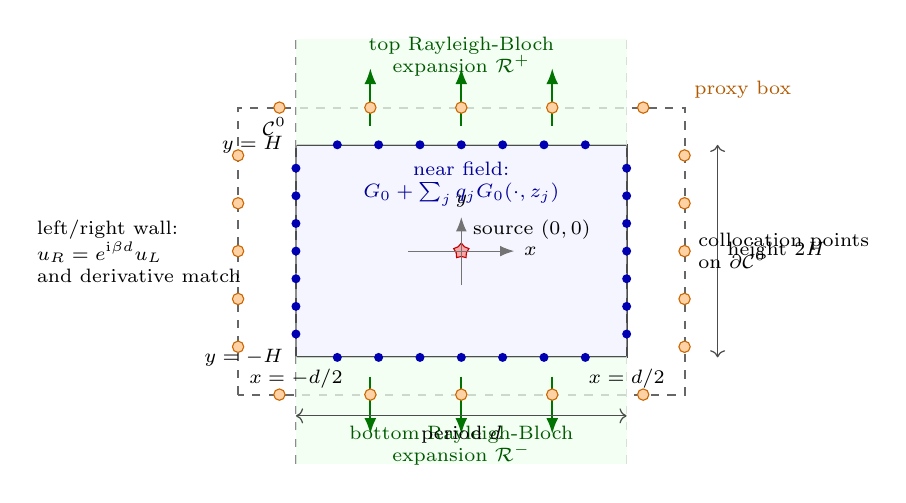
\begin{tikzpicture}[
    x=2.1cm,
    y=1.35cm,
    every node/.style={font=\scriptsize},
    cell/.style={draw=black!70, line width=0.75pt, fill=blue!4},
    proxybox/.style={draw=black!60, dashed, line width=0.75pt},
    wall/.style={draw=black!45, dashed, line width=0.55pt},
    colloc/.style={circle, fill=blue!70!black, inner sep=1.15pt},
    proxy/.style={circle, draw=orange!80!black, fill=orange!35, inner sep=1.45pt},
    source/.style={star, star points=5, draw=red!75!black, fill=red!35,
      minimum size=5.8pt, inner sep=0pt},
    dim/.style={<->, draw=black!70, line width=0.45pt},
    ray/.style={-{Latex[length=2mm]}, draw=green!45!black, line width=0.7pt},
    note/.style={align=center, font=\scriptsize}
  ]
    % Coordinates use normalized d=2, H=1 in drawing units:
    % central cell [-1,1] x [-1,1], proxy box [-1.35,1.35] x [-1.35,1.35].
    \draw[cell] (-1,-1) rectangle (1,1);
    \draw[proxybox] (-1.35,-1.35) rectangle (1.35,1.35);

    % Only the vertical side walls are extended in y.
    \draw[wall] (-1,-2.0) -- (-1,2.0);
    \draw[wall] (1,-2.0) -- (1,2.0);

    % Rayleigh-Bloch regions.
    \fill[green!6, opacity=0.75] (-1,1) rectangle (1,2.0);
    \fill[green!6, opacity=0.75] (-1,-2.0) rectangle (1,-1);
    \draw[ray] (-0.55,1.18) -- (-0.55,1.72);
    \draw[ray] (0.0,1.18) -- (0.0,1.72);
    \draw[ray] (0.55,1.18) -- (0.55,1.72);
    \draw[ray] (-0.55,-1.18) -- (-0.55,-1.72);
    \draw[ray] (0.0,-1.18) -- (0.0,-1.72);
    \draw[ray] (0.55,-1.18) -- (0.55,-1.72);
    \node[note, green!35!black] at (0,1.83)
      {top Rayleigh-Bloch\\expansion \(\Rup\)};
    \node[note, green!35!black] at (0,-1.83)
      {bottom Rayleigh-Bloch\\expansion \(\Rdn\)};

    % Source and axes.
    \node[source] at (0,0) {};
    \node[above right=1pt] at (0,0) {source \((0,0)\)};
    \draw[-{Latex[length=1.8mm]}, draw=black!55] (-0.32,0) -- (0.32,0);
    \draw[-{Latex[length=1.8mm]}, draw=black!55] (0,-0.32) -- (0,0.32);
    \node[right] at (0.32,0) {$x$};
    \node[above] at (0,0.32) {$y$};

    % Proxy sources on the dashed proxy box.
    \foreach \x in {-1.1,-0.55,0,0.55,1.1} {
      \node[proxy] at (\x,1.35) {};
      \node[proxy] at (\x,-1.35) {};
    }
    \foreach \y in {-0.9,-0.45,0,0.45,0.9} {
      \node[proxy] at (-1.35,\y) {};
      \node[proxy] at (1.35,\y) {};
    }

    % Collocation points on central-cell boundary.
    \foreach \y in {-0.78,-0.52,-0.26,0,0.26,0.52,0.78} {
      \node[colloc] at (-1,\y) {};
      \node[colloc] at (1,\y) {};
    }
    \foreach \x in {-0.75,-0.5,-0.25,0,0.25,0.5,0.75} {
      \node[colloc] at (\x,1) {};
      \node[colloc] at (\x,-1) {};
    }

    % Labels.
    \node[above left] at (-1,1) {\(\Czero\)};
    \node[above right, orange!70!black] at (1.35,1.35) {proxy box};
    \node[note, blue!60!black] at (0,0.63)
      {near field:\\\(\Gfree+\sum_j q_j\Gfree(\cdot,z_j)\)};
    \node[below] at (-1,-1.02) {$x=-d/2$};
    \node[below] at (1,-1.02) {$x=d/2$};
    \node[left] at (-1.02,1) {$y=H$};
    \node[left] at (-1.02,-1) {$y=-H$};

    % Dimension braces.
    \draw[dim] (-1,-1.55) -- (1,-1.55);
    \node[below] at (0,-1.55) {period \(d\)};
    \draw[dim] (1.55,-1) -- (1.55,1);
    \node[right] at (1.55,0) {height \(2H\)};

    \node[note, align=left] at (-1.95,0)
      {left/right wall:\\\(u_R=e^{\ii\beta d}u_L\)\\and derivative match};
    \node[note, align=left] at (1.95,0)
      {collocation points\\on \(\partial\Czero\)};
  \end{tikzpicture}
\end{frame}

\begin{frame}{Rayleigh-Bloch Notation}
  \small
  For a source \(s=(x_s,y_s)\), define relative coordinates
  \[
    X=x-x_s,\qquad Y=y-y_s,
  \]
  and Rayleigh-Bloch horizontal wavenumbers
  \[
    \beta_m=\beta+\frac{2\pi m}{d},
    \qquad
    \gamma_m=\sqrt{k^2-\beta_m^2}.
  \]
  The branch of \(\gamma_m\) is chosen so that propagating modes are
  outgoing and evanescent modes decay away from the artificial boundaries.

  \begin{block}{x-periodic convention}
    The phase \(e^{\ii\beta d}\) is attached to translations in \(x\).
    The Rayleigh-Bloch modes propagate or decay in the transverse
    \(y\)-direction.
  \end{block}
\end{frame}

\begin{frame}{Piecewise Ansatz}
  \footnotesize
  With \(X=x-x_s\) and \(Y=y-y_s\), the approximation has three regions:

  \[
  \Gqp(x,y;s)\approx
  \begin{cases}
  \displaystyle
  \sum_{m=-M}^{M} c_m^+\,
  e^{\ii\beta_m X}e^{\ii\gamma_m(Y-H)},
  & Y>H,\\[0.45em]
  \displaystyle
  \Gfree((x,y),s)+
  \sum_{j=1}^{\Np} q_j\,\Gfree((x,y),z_j),
  & |Y|\le H,\\[0.45em]
  \displaystyle
  \sum_{m=-M}^{M} c_m^-\,
  e^{\ii\beta_m X}e^{-\ii\gamma_m(Y+H)},
  & Y<-H.
  \end{cases}
  \]

  \vspace{0.3em}
  The fundamental-solution plus Rayleigh-expansion construction follows the
  meshless quasi-periodic scattering strategy of Luan--Sun--Zhuang
  \cite{LuanSunZhuang2019}, adapted here to a Green-function source.
\end{frame}

\begin{frame}{Collocation Equations}
  \small
  The unknowns are proxy strengths \(q_j\) and upward/downward Rayleigh
  coefficients \(c_m^\pm\).  They are determined by boundary collocation:

  \begin{block}{Left/right x-quasiperiodicity}
    At matched points on \(x=\pm d/2\),
    \[
      u(d/2,y)=e^{\ii\beta d}u(-d/2,y),
      \qquad
      \partial_x u(d/2,y)=e^{\ii\beta d}\partial_x u(-d/2,y).
    \]
  \end{block}

  \begin{block}{Top/bottom artificial boundaries}
    On \(y=H\), match the near-field expression to \(\Rup\) in value and
    \(\partial_y\).  On \(y=-H\), match it to \(\Rdn\) in value and
    \(\partial_y\).
  \end{block}

  \vspace{0.2em}
  The proxy sources represent only the bounded near-field correction.  The
  top and bottom unbounded regions are not meshed or truncated; they are
  represented by Rayleigh-Bloch modes.
\end{frame}

\begin{frame}{Connection to the Current Code}
  \small
  \begin{center}
  \renewcommand{\arraystretch}{1.12}
  \begin{tabular}{ll}
    \hline
    code object & mathematical role\\
    \hline
    \texttt{kernel.precomp\_proxy} &
    solve the collocation least-squares system\\
    \texttt{kernel.qpgreen\_mfs} &
    evaluate the piecewise representation at target points\\
    \texttt{kernel.qpgreen\_mfs\_pairmat} &
    build target-source matrices for \(A_{\mathrm{QP}}\) assembly\\
    \texttt{pars1.d, pars1.beta, pars1.k} &
    \(d,\beta,k\) in the x-periodic Green function\\
    \texttt{pars2.H} &
    half-height of \(\Czero\) in the transverse \(y\) direction\\
    \texttt{pars2.M\_pw} &
    Rayleigh half-truncation \(M\)\\
    \texttt{pars2.N\_proxy\_edge} &
    proxy source density on the dashed box\\
    \hline
  \end{tabular}
  \end{center}

  \vspace{0.2em}
  In the default x-periodic benchmark, \(d=1\), \(H=0.5\),
  \(M=25\), and \(N_{\mathrm p}=320\) proxy sources are placed on the
  enclosing proxy box.
\end{frame}

\section{Rayleigh Truncation Check}

\begin{frame}{Rayleigh Truncation: M-sweep on Linton Benchmark}
  \scriptsize
  A lightweight tuning experiment uses only the Linton Table 4 single-point
  benchmark
  \[
    kd=2,\qquad \beta d=3,\qquad d=1,\qquad H=0.5,
  \]
  with the same source/target point and Ewald reference as before.

  \begin{itemize}
    \item Only the Rayleigh half-truncation \(M\) is changed.
    \item \(N_{\mathrm p}=320\), proxy placement, and collocation placement
    are fixed.
    \item Unknown Rayleigh coefficients: \(2(2M+1)\).
    \item Goal: test whether the previous default \(M=25\) is necessary.
  \end{itemize}

  \vspace{0.1em}
  \centering
  \SafeIncludeGraphics[
    width=0.70\textwidth,
    height=0.30\textheight,
    keepaspectratio
  ]{figures/linton_M_sweep_error.pdf}
\end{frame}

\begin{frame}{Observation: Small M is Enough for H = 0.5}
  \scriptsize
  \begin{center}
  \renewcommand{\arraystretch}{1.12}
  \begin{tabular}{rrrrr}
    \hline
    \(M\) & modes \(2M+1\) & unknowns & equations
      & \(|G_{\mathrm{MFS}}-G_{\mathrm{Ewald}}|\)\\
    \hline
    4  & 9  & 338 & 960 & \(1.9590{\times}10^{-7}\)\\
    6  & 13 & 346 & 960 & \(8.0251{\times}10^{-8}\)\\
    8  & 17 & 354 & 960 & \(6.5370{\times}10^{-8}\)\\
    10 & 21 & 362 & 960 & \(1.9584{\times}10^{-7}\)\\
    12 & 25 & 370 & 960 & \(1.0305{\times}10^{-7}\)\\
    25 & 51 & 422 & 960 & \(2.4016{\times}10^{-8}\)\\
    \hline
  \end{tabular}
  \end{center}

  \vspace{0.25em}
  The sweep is not monotone, but the practical scale is clear: \(M=6\)--12
  already gives \(10^{-7}\)-level agreement with the Ewald benchmark, while
  \(M=25\) gives the smallest error in this run, about \(2.4{\times}10^{-8}\).
  Thus \(M=25\) improves the single-point value, but not by orders of
  magnitude relative to \(M=8\) or \(M=12\).

  \vspace{0.25em}
  A simple scale estimate explains why small \(M\) can work here:
  \[
    |\beta_m|\sim 2\pi |m|,\qquad
    e^{-|\beta_m|H}\sim e^{-2\pi |m|H}.
  \]
  For \(H=0.5\), each additional Fourier order contributes roughly another
  factor \(e^{-\pi}\approx 4.3{\times}10^{-2}\).  This is only a Rayleigh
  tail estimate, not a complete MFS error bound.
\end{frame}

\section{Linton Table Benchmarks}

\begin{frame}{Benchmark Against Linton Tables 2--4}
  \scriptsize
  Linton's Tables 2--4 give 10-digit reference values for the
  quasi-periodic Green function at
  \[
    X_{\mathrm L}/d=0,\qquad Y_{\mathrm L}/d=0.01,
  \]
  for three pairs of \((kd,\beta d)\) \cite{Linton1998}.

  \begin{block}{Coordinate convention}
    Linton periodicizes the \(Y\)-direction.  The project qpgreen is
    x-periodic, so the table point is evaluated with
    \[
      (x\text{-periodic separation},\,y\text{-transverse separation})
      =
      (Y_{\mathrm L},\,X_{\mathrm L}).
    \]
  \end{block}

  We compare the project MFS qpgreen with an x-periodic Ewald benchmark.
  The Linton printed value is kept as an external sign-convention check.

  \begin{block}{MFS parameters used below}
    Table-4-tuned setting:
    \(H=0.6,\ M=16,\ N_{\mathrm p}=160,\ \mathrm{proxy\ dist}=0.15,\)
    and \(N_{\mathrm{side}}=N_{\mathrm{top}}=160\).
  \end{block}
\end{frame}

\begin{frame}{MFS Parameters for the Linton Table Run}
  \scriptsize
  The following MFS parameters are used for all three Linton table cases in
  the next slides.  Only \(k\) and \(\beta\) change from table to table.

  \vspace{0.1em}
  \begin{center}
  \renewcommand{\arraystretch}{1.04}
  \begin{tabular}{lll}
    \hline
    parameter & value & role\\
    \hline
    \(d\) & \(1\) & x-period\\
    \(H\) & \(0.6\) & half-height of the matching box \( [-d/2,d/2]\times[-H,H]\)\\
    \(M\) & \(16\) & Rayleigh half-truncation, \(m=-M,\ldots,M\)\\
    \(2M+1\) & \(33\) & Rayleigh modes above and below the box\\
    \(N_{\mathrm p}\) & \(160\) & total proxy sources on the enclosing proxy box\\
    proxy distance & \(0.15\) & offset from \(\Czero\) to the proxy box\\
    \(N_{\mathrm{side}}\) & \(160\) & collocation points on each left/right wall\\
    \(N_{\mathrm{top}}\) & \(160\) & collocation points on each top/bottom boundary\\
    \hline
  \end{tabular}
  \end{center}

  \vspace{0.1em}
  Unknowns:
  \(N_{\mathrm p}+2(2M+1)=160+66=226\).
  Collocation equations:
  \(2N_{\mathrm{side}}+4N_{\mathrm{top}}=320+640=960\).
  The side equations enforce left/right value and \(\partial_x\)
  quasiperiodicity; the top/bottom equations enforce value and
  \(\partial_y\) Rayleigh matching.
\end{frame}

\begin{frame}{Accuracy and Sign Convention}
  \scriptsize
  Project kernels use \(\ii H_0^{(1)}/4\), while Linton's printed values use
  the opposite Green-function sign.  Therefore the diagnostic checks
  \[
    G_{\mathrm{Linton}}\approx -G_{\mathrm{project}}.
  \]

  \vspace{0.25em}
  \begin{center}
  \renewcommand{\arraystretch}{1.12}
  \begin{tabular}{rrrrr}
    \hline
    Table & \(kd\) & \(\beta d\) & \(|G_{\mathrm{MFS}}-G_{\mathrm{Ewald}}|\)
      & relative error\\
    \hline
    2 & \(2\) & \(\sqrt2\) & \(4.1038{\times}10^{-9}\) & \(7.0976{\times}10^{-9}\)\\
    3 & \(10\) & \(5\sqrt2\) & \(4.5691{\times}10^{-9}\) & \(1.1550{\times}10^{-8}\)\\
    4 & \(2\) & \(3\) & \(1.1140{\times}10^{-9}\) & \(1.4624{\times}10^{-9}\)\\
    \hline
  \end{tabular}
  \end{center}

  \vspace{0.35em}
  \begin{itemize}
    \item Sign diagnostic from the run:
    \[
      \|G_{\mathrm{Ewald}}-G_{\mathrm{Linton}}\|=2.0698,
      \qquad
      \|-G_{\mathrm{Ewald}}-G_{\mathrm{Linton}}\|=7.3545{\times}10^{-11}.
    \]
    \item Thus the comparison MFS vs Ewald is made in the project sign
    convention; Linton's values validate the Ewald reference up to sign.
    \item Compared with the previous \(H=0.5,M=25,N_{\mathrm p}=320\)
    table run, the absolute errors improve by about \(3.4\times\),
    \(3.2\times\), and \(21.6\times\) for Tables 2--4.
  \end{itemize}
\end{frame}

\begin{frame}{Representative Values}
  \scriptsize
  The following are project-sign values from the benchmark output.  Linton's
  10-digit references are the negatives of the listed Ewald values.

  \vspace{0.2em}
  \begin{center}
  \renewcommand{\arraystretch}{1.15}
  \begin{tabular}{rll}
    \hline
    Table & Ewald value & MFS value\\
    \hline
    2 &
    \(0.4595298795+0.3509130869\ii\) &
    \(0.4595298756+0.3509130883\ii\)\\
    3 &
    \(0.3538172307+0.1769332383\ii\) &
    \(0.3538172336+0.1769332417\ii\)\\
    4 &
    \(0.7617463954+0.0006387129\ii\) &
    \(0.7617463964+0.0006387135\ii\)\\
    \hline
  \end{tabular}
  \end{center}

  \vspace{0.4em}
  \begin{block}{Interpretation}
    The Table-4-tuned MFS parameters improve all three Linton table cases.
    The two non-tuned cases still land near a few \(10^{-9}\), while the
    tuned Table 4 point reaches \(1.1{\times}10^{-9}\).
  \end{block}
\end{frame}

\begin{frame}{Runtime Comparison}
  \scriptsize
  Timing is from the same run as the accuracy table.  The MFS total is the
  benchmark wrapper wall time; the precomp/eval columns isolate the kernel
  costs.  Importantly,
  \[
    \texttt{kernel.qpgreen\_mfs}
    \quad\text{computes value, gradient, and Hessian,}
  \]
  while the benchmark Ewald helper currently computes only the function
  value.

  \vspace{0.15em}
  \begin{center}
  \renewcommand{\arraystretch}{1.12}
  \begin{tabular}{rrrrrr}
    \hline
    Table & Ewald value-only & MFS total & MFS precomp & MFS eval & total ratio\\
    \hline
    2 & \(0.003246\) & \(0.382164\) & \(0.235503\) & \(0.003260\) & \(117.7\)\\
    3 & \(0.001181\) & \(0.356029\) & \(0.238551\) & \(0.000791\) & \(301.5\)\\
    4 & \(0.000599\) & \(0.402536\) & \(0.245741\) & \(0.000560\) & \(672.1\)\\
    \hline
  \end{tabular}
  \end{center}

  \vspace{0.25em}
  \begin{itemize}
    \item For a single target, MFS is dominated by the reusable
    least-squares precomputation.
    \item The evaluation-only MFS cost is comparable to Ewald value-only
    even though MFS also returns first and second derivatives.
    \item The tuned setting uses \(226\) unknowns instead of the previous
    \(422\), so the single-point error improves while the precomputation
    is also smaller.
    \item For \(A_{\mathrm{QP}}\) assembly, the precomputation is amortized
    over many target-source pairs; the present Ewald timings are a lower
    bound because derivative and Hessian Ewald formulas are not yet included.
  \end{itemize}
\end{frame}

\section{Grid Benchmark in \texorpdfstring{\(\Czero\)}{C0}}

\begin{frame}{Cell-grid Error Benchmark}
  \small
  The grid experiment compares MFS and Ewald values on
  \[
    \Czero=[-d/2,d/2]\times[-H,H],
    \qquad
    d=1,\quad H=0.5,
  \]
  with the source at \((0,0)\).  The source grid point is excluded.

  \begin{block}{What this error means}
    The plotted error is
    \[
      |G_{\mathrm{MFS}}-G_{\mathrm{Ewald}}|,
    \]
    where \(G_{\mathrm{Ewald}}\) is the benchmark implementation following
    Linton's Ewald formula, converted to the project x-periodic convention.
    It is \textbf{not} an error against a known closed-form exact value.
  \end{block}

  \vspace{0.1em}
  The goal is to test whether the MFS representation tracks the Ewald
  reference throughout \(\Czero\), away from the singular source point.
\end{frame}

\begin{frame}{Absolute Error Contour}
  \centering
  \SafeIncludeGraphics[
    width=0.76\textwidth,
    height=0.70\textheight,
    keepaspectratio
  ]{../../benchmark/output/figures/qpgreen_grid_logerr_20260527_111712.png}

  \vspace{0.2em}
  \scriptsize
  Contour of \(\log_{10}|G_{\mathrm{MFS}}-G_{\mathrm{Ewald}}|\) on
  \(101\times81\) grid points in \(\Czero\).  The source-near grid point is
  excluded from the statistic and shown as the marked singular point.
\end{frame}

\begin{frame}{Grid Error and Runtime Summary}
  \scriptsize
  Default benchmark parameters:
  \(k=2\), \(\beta=\sqrt2\), \(d=1\), \(H=0.5\),
  \(N_{\mathrm p}=320\), \(M=25\), and \(101\times81\) grid points.

  \vspace{0.2em}
  \begin{center}
  \renewcommand{\arraystretch}{1.12}
  \begin{tabular}{lr}
    \hline
    statistic & value\\
    \hline
    valid grid points & \(8180\)\\
    source-excluded points & \(1\)\\
    max absolute error & \(6.9904{\times}10^{-8}\)\\
    median absolute error & \(3.1418{\times}10^{-8}\)\\
    RMS absolute error & \(3.5435{\times}10^{-8}\)\\
    max relative error & \(1.8888{\times}10^{-7}\)\\
    \hline
  \end{tabular}
  \qquad
  \begin{tabular}{lr}
    \hline
    timing & seconds\\
    \hline
    Ewald value-only total & \(3.941659\)\\
    MFS total & \(2.782947\)\\
    MFS precomputation & \(0.570537\)\\
    MFS grid evaluation & \(2.210147\)\\
    MFS total / Ewald total & \(0.706034\)\\
    MFS eval-only / Ewald total & \(0.560715\)\\
    \hline
  \end{tabular}
  \end{center}

  \vspace{0.3em}
  The contour and statistics show that, inside \(\Czero\), MFS agrees with
  the Ewald reference at the \(10^{-7}\)--\(10^{-8}\) level.  As before,
  MFS evaluates value, gradient, and Hessian, while this Ewald timing is
  value-only.
\end{frame}

\section{References}

\begin{frame}[allowframebreaks]{References}
  \bibliographystyle{plain}
  \bibliography{pre3}
\end{frame}

\end{document}
